% This file is part of Bachelorarbeit

% Bachelorarbeit is free software: you can redistribute it and/or modify
% it under the terms of the GNU General Public License version 3 as published by
% the Free Software Foundation.

% Bachelorarbeit is distributed in the hope that it will be useful,
% but WITHOUT ANY WARRANTY; without even the implied warranty of
% MERCHANTABILITY or FITNESS FOR A PARTICULAR PURPOSE.  See the
% GNU General Public License for more details.

% You should have received a copy of the GNU General Public License
% along with Foobar. If not, see <http://www.gnu.org/licenses/>.
\section{Basis}
Als Basis der Arbeit wurde der quelloffene VPN-Dienst strongSwan gewählt,
welcher von der Hochschule für Technik Rapperswill entwickelt wird.
Um die Pakete vom Kernelspace in Empfang nehmen zu können, wird der quelloffene
TAP-Gerätetreiber von OpenVPN Technologies, Inc. genutzt. Dieser stellt funktionierende
und nutzbare TUN- und TAP-Geräte bereit, mit denen gearbeitet werden kann.
Für die Verarbeitung der Pakete wird die in strongSwan integrierte Bibliothek libipsec,
das Plugin kernel-libipsec, sowie bestehende Teile von libstrongswan
aus strongSwan genutzt.

\subsection{Bestehende Implementierungen für Windows}

In \autoref{sec:appendix} ist eine Auflistung aller mir bekannten IPsec-Clients für Windows,
inklusive Matrizen der jeweils unterstützten Algorithmen und Verfahren in den ISAKMP-
und IKE-Standards.

\subsection{strongSwan}
strongSwan implementiert einen beträchtlichen Teil der Funktionalität der \acp{RFC} für IKEv2\footcite{_ipsecstandards_2016}.
Die Software ist multithreaded und in Objektorientiertem C geschrieben.
Die Grundlage wurde von Martin Willi und Jan Hutter in ihrer Diplomarbeit im Jahr 2005 gelegt\footcite[][]{jan_hutter_strongswan_2005}.
\subsubsection{charon}
Charon ist der Daemon, der in der Diplomarbeit\footcite[][]{jan_hutter_strongswan_2005} entwickelt wurde.
Er arbeitet parallel und wurde in objektorientiertem C geschrieben, so wie die Software Xine.
Intern werden verschiedene Bibliotheken genutzt, angefangen von libstrongswan bis zu libcharon.
Es existieren verschiedene Versionen von charon für verschiedene Zwecke, zum Beispiel
charon-svc. charon-svc ist eine Version von charon, die als Dienst auf Windows genutzt werden kann.

Jegliche Funktionalität von strongSwan ist in Form einer Bibliothek untergebracht und in objektorientiertem
C geschrieben. Das ermöglicht es die Namensräume in strongSwan relativ frei zu halten
und Objekte gleichen Typs gleich zu behandeln, sowie die Duplikation von kurzem Code
zu vermeiden.

Ein Beispiel dafür ist libstrongswan, welche unter anderem 
allgemeine Datenstrukturen wie Linked Lists, Arrays und Hashtables, sowie Code für TUN-Geräte und
Multithreading implementiert.

% Mehr Informationen?
\subsubsection{Userspace processing}
Userspace processing wurde in charon von Guiliano Grassi und Ralf Sager für Android implementiert,
um die Entwicklung der strongSwan-App für Android zu ermöglichen. Auf Android ist kernelspace processing
von \ac{IPsec}-Paketen nicht möglich, da die Privilegien der Anwendung das nicht erlauben.

Um Userspace Processing von \ac{IPsec}-Paketen zu implementieren benötigt
die Anwendung, die die Pakete verarbeiten soll, Zugriff auf die Pakete und muss,
damit die darin enthaltenen Pakete an den Zielort weitergeleitet werden können,
eine Möglichkeit haben sie an den Kernel zum Routing zu übergeben. In der Regel wird
dies mit TUN- oder TAP-Geräten bewerkstelligt, die einen virtuellen Netzwerkadapter
darstellen. Am einen Ende hängt der Kernel mit seiner Routing-Engine und den Firewallregeln,
am anderen Ende hängt die Anwendung, die Pakete auf einen \ac{FD} oder ein Handle schreibt
und davon liest.

Pakete, die in den Adapter gesendet werden werden von der Anwendung empfangen
und Pakete, die in das Handle geschrieben werden, tauchen auf dem Adapter auf Seiten
des Betriebssystems auf.

\paragraph{OpenVPN TAP-Treiber}
Der OpenVPN-Tap-Treiber ist unter den Namen ''TAP-Windows'' bekannt und wurde von
OpenVPN Technologies, Inc. für den Einsatz mit OpenVPN entwickelt.
Der Treiber stellt unter Windows ein Ethernet-Gerät dar, inklusive Kollisionsdomäne.
Dies ist für dein Einsatz mit \ac{IPsec} etwas unbeholfen, da \ac{IPsec} \ac{IP}-Pakete
überträgt und keine Ethernet-Rahmen.
Der Treiber unterstützt, wie OpenVPN, das Tunneln von Ethernet-Frames jedoch (TAP-Modus).
Der Treiber bewerkstelligt das, indem er den Ethernet-Rahmen eines eingehenden Pakets vom
Host verwirft und nur das IP-Paket weiterleitet. Vice Versa ergänzt er IP-Pakete, die er von
der Software erhält um einen Ethernet-Rahmen. Um über den Adapter kommunizieren zu können
stellt der Treiber einen virtuellen Router bereit, dessen \ac{IP}-Adresse, wie die lokale  und
die entfernte IP-Adresse(n) konfigurierbar ist.
Der Treiber reagiert nicht auf jede ARP-Anfrage, sondern nur auf solche, bei denen
die Quelladresse im ARP-Request der lokalen konfigurierten gleicht, sowie die erfragte Adresse
der konfigurierten entfernten Adresse (oder einer der Entfernten, falls ein gesamtes Netzwerk
als entfernte IP konfiguriert wurde) gleicht.
Die MAC-Adresse des virtuellen Routers hängt von der GUID des Adapters ab, welche zufällig ist
und bei der Erstellung des Adapters initialisiert wird. Die MAC-Adresse kann 
auch über die Registry verändert werden.

Um mit dem virtuellen Adapter kommunizieren zu können, wird ein Handle mit dem Gerät
geöffnet, über das dann asynchron gelesen und geschrieben werden kann.

\paragraph{Betriebsmodi}
Der TAP-Treiber beherrscht drei verschiedene Betriebsmodi für verschiedene Zwecke.
Laut dem Quellcode des Treibers ist der Point-To-Point-Modus veraltet.
\begin{description}
\item [TUN-Modus] Im TUN-Modus schneidet der Treiber den Ethernet-Rahmen um das 
IP-Paket ab und reicht das Paket über das Handle an die Software weiter. 
Pakete, die an den Treiber gegeben werden, werden um einen Ethernet-Rahmen
ergänzt, bei dem die Zieladresse die MAC-Adresse des virtuellen Adapters ist 
und die Quelladresse die MAC-Adresse des virtuellen Routers.
In diesem Modus existiert eine lokale IP-Adresse, ein virtueller Router und 
ein entferntes Netzwerk.
% remote subnet, local subnet, local IP
\item [TAP-Modus] Im TAP-Modus kopiert der Treiber jeden Ethernet-Paket zwischen 
Anwendung und Gerät.
% remote subnet, local subnet, local IP
\item [Point-To-Point-Modus] Im Point-To-Point-Modus existiert eine lokale IP 
und eine entfernte IP. Empfangene Ethernet-Frames werden entfernt und nur
das enthaltene IP-Paket weitergereicht.
\end{description}

\paragraph{libipsec}
libipsec ist eine Bibliothek, die IPsec im Tunnelmodus implementiert.
Sie ist Teil des strongSwan-Quellcodes. Sie wird für die Verarbeitung von IP-Paketen
in der Regel auf Systemen genutzt, die keine (funktionierenden) IPsec-Implementierung
enthalten.

libipsec besteht aus zwei Komponenten: Einerseits die Bibliothek, die die SAD und die SPD
implementiert, sowie die Verarbeitung (libipsec) und ein Plugin, welches ein Kernel-Interface
für das Verwalten der \ac{SAD} und \ac{SPD} emuliert (kernel-libipsec).

libipsec empfängt und sendet Pakete über die gleichen Sockets, den der restliche Teil
des Daemons benutzt, um mit anderen IKE-Peers zu kommunizieren. Das sind Sockets,
die auf UDP mit Port 500 und 4500 gebunden sind; die IKE-Standardports.
libipsec unterstützt die Verarbeitung von ESPINUDP-Paketen, sowie von normalen ESP-Paketen,
da sie sich strukturell nur gering unterscheiden. Jedoch wird aufgrund der Tatsache,
dass mit den gegebenen Sockets kommuniziert wird, UDP-Encapsulation forciert.
Um ESP-Pakete verschicken zu können, müsste ein Socket geöffnet werden der das
verschicken von solchen Paketen erlauben würde. Das ist jedoch auf der Plattform,
für die die Bibliothek ursprünglich geschaffen wurde (Android) nicht erlaubt, da
die Privilegien der Anwendung dort sehr beschränkt sind.

Prinzipiell wäre es jedoch möglich dies zu implementieren. Dafür müsste ein
raw-Socket geöffnet werden, über den rein IP gesprochen wird.
\begin{figure}
\centering
%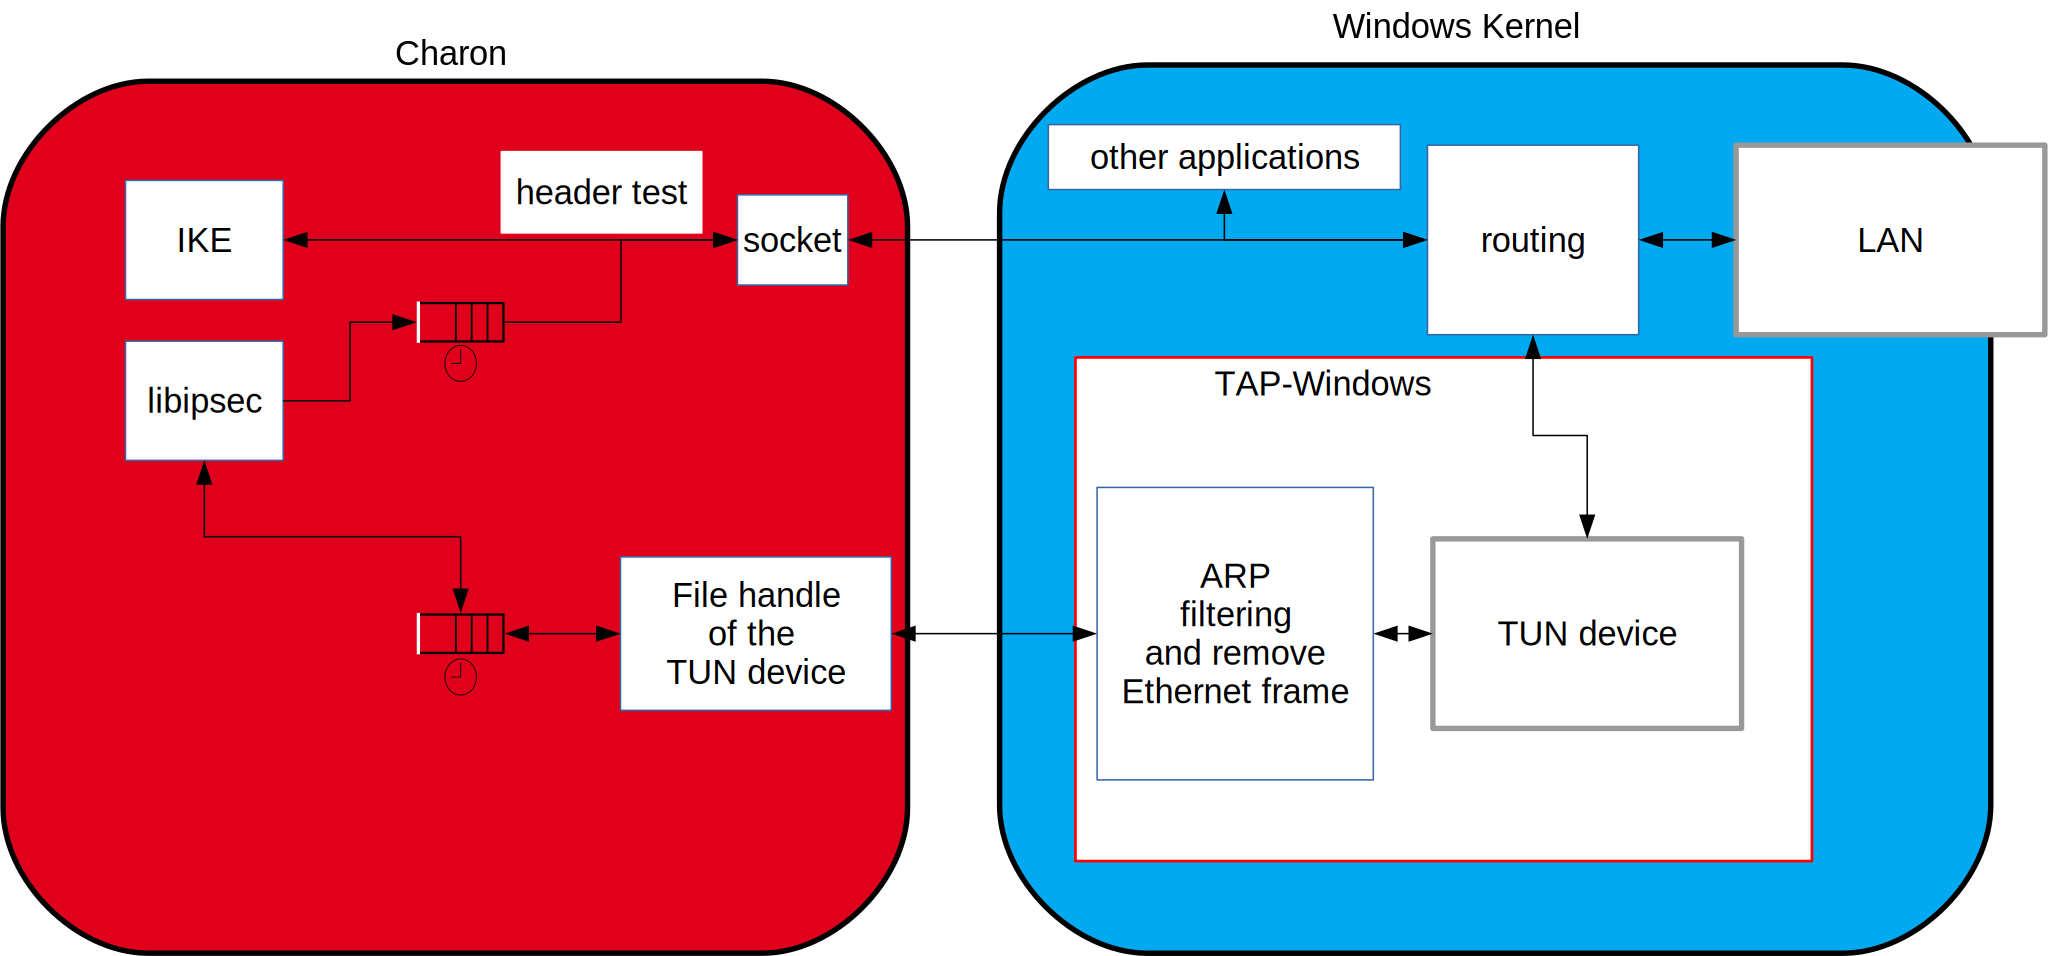
\includepdf[pages=1,pagecommand={}]{Diagram.pdf}
%\def\svgwidth{\columnwidth}
%\includesvg{Diagram}
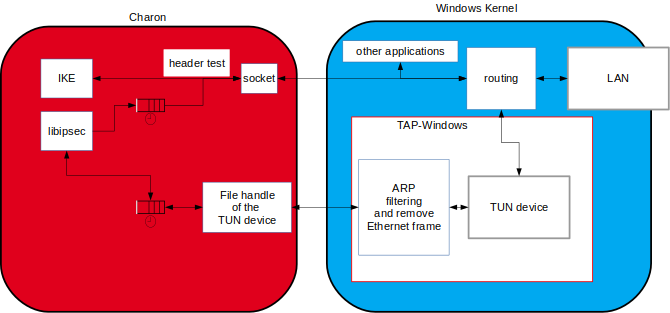
\includegraphics[width=\textwidth]{Diagram.png}
\caption{Strukturdiagramm von libipsec auf Windows }
\end{figure}

%demultiplexing NON-ESP marker, SPI
\subparagraph{libstrongswan}
libstrongswan ist eine interne Bibliothek von strongSwan, die von den verschiedenen
Versionen von charon geladen wird, um diverse Funktionalität zu erhalten, wie
Linked-Lists, Hashtables, Arrays, sowie die Funktionen um TUN-Geräte zu erstellen und zu öffnen.

Der Code für das lesen und schreiben von Paketen existiert bereits für Linux, Mac OSX
und FreeBSD.
Die Operationen basieren dabei auf File Descriptors, welche mit poll() multiplext nach
Daten abgefragt werden.
